
\chapter{Asymptotic Notation}

\section{Big-O }

\dfn{Let $f(n)$ and $g(n)$ be functions from the set of positive integers to the set of positive real numbers. We say that $f(n)$ is $O(g(n))$ if there exist positive constants $c$ and $n_0$ such that $0 \leq f(n) \leq cg(n)$ for all $n \geq n_0$.}

\begin{figure}[h]
	\centering
	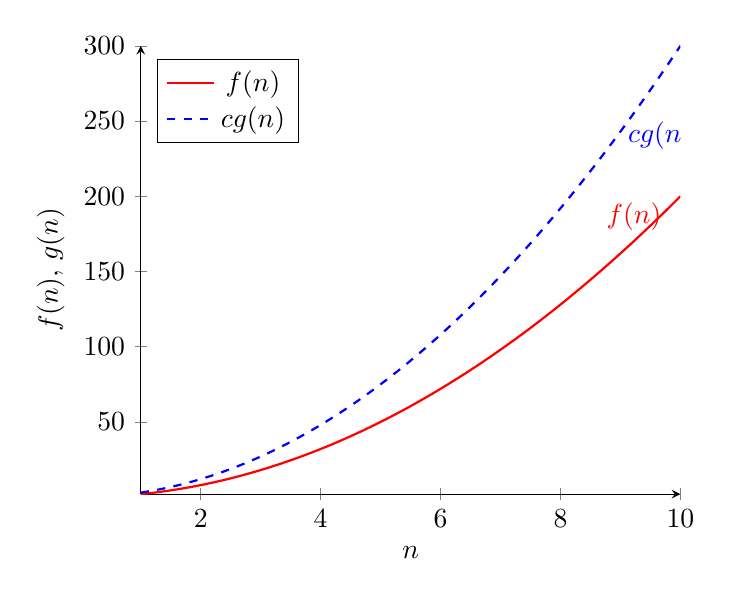
\begin{tikzpicture}
		\begin{axis}[
				domain=1:10,
				samples=100,
				axis x line=bottom,
				axis y line=left,
				xlabel=$n$,
				ylabel={$f(n)$, $g(n)$},
				legend pos=north west
			]
			\addplot[thick, red] {2*x^2} node[pos=0.85, above] {$f(n)$};
			\addplot[thick, blue, dashed] {3*x^2} node[pos=0.8, right] {$cg(n)$};
			\legend{$f(n)$, $cg(n)$}
		\end{axis}
	\end{tikzpicture}
	\caption{Graph showing $f(n) = O(g(n))$}
\end{figure}

\pagebreak

\section{Big-$\Omega$}

\dfn{Let $f(n)$ and $g(n)$ be functions from the set of positive integers to the set of positive real numbers. We say that $f(n)$ is $\Omega(g(n))$ if there exist positive constants $c$ and $n_0$ such that $0 \leq cg(n) \leq f(n)$ for all $n \geq n_0$.}

\begin{figure}[h]
	\centering
	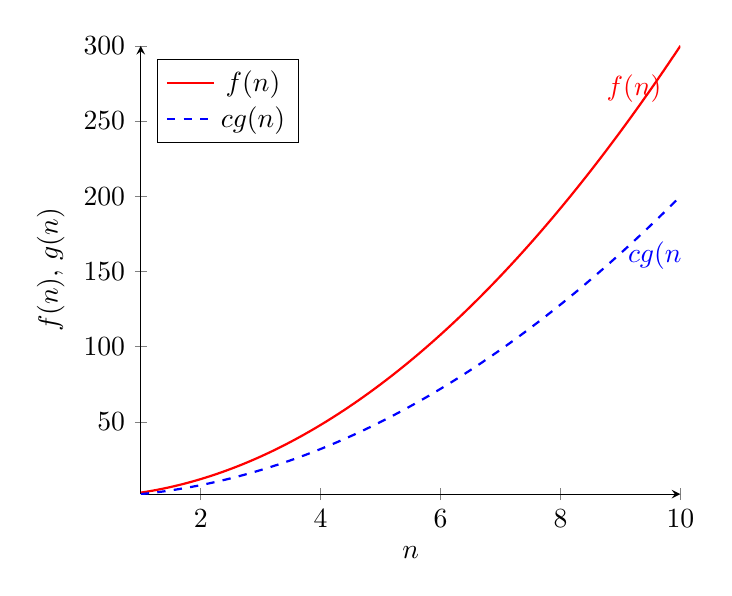
\begin{tikzpicture}
		\begin{axis}[
				domain=1:10,
				samples=100,
				axis x line=bottom,
				axis y line=left,
				xlabel=$n$,
				ylabel={$f(n)$, $g(n)$},
				legend pos=north west
			]
			\addplot[thick, red] {3*x^2} node[pos=0.85, above] {$f(n)$};
			\addplot[thick, blue, dashed] {2*x^2} node[pos=0.8, right] {$cg(n)$};
			\legend{$f(n)$, $cg(n)$}
		\end{axis}
	\end{tikzpicture}
	\caption{Graph showing $f(n) = \Omega(g(n))$}
\end{figure}

\pagebreak

\section{Big-$\Theta$}

\dfn{Let $f(n)$ and $g(n)$ be functions from the set of positive integers to the set of positive real numbers. We say that $f(n)$ is $\Theta(g(n))$ if there exist positive constants $c_1$, $c_2$ and $n_0$ such that $0 \leq c_1g(n) \leq f(n) \leq c_2g(n)$ for all $n \geq n_0$.}

\begin{figure}[h]
	\centering
	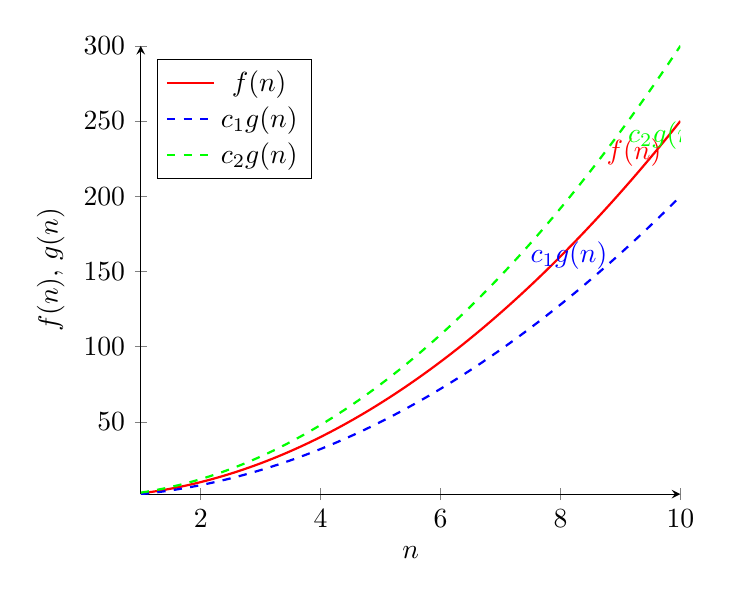
\begin{tikzpicture}
		\begin{axis}[
				domain=1:10,
				samples=100,
				axis x line=bottom,
				axis y line=left,
				xlabel=$n$,
				ylabel={$f(n)$, $g(n)$},
				legend pos=north west
			]
			\addplot[thick, red] {2.5*x^2} node[pos=0.85, above] {$f(n)$};
			\addplot[thick, blue, dashed] {2*x^2} node[pos=0.8, left] {$c_1g(n)$};
			\addplot[thick, green, dashed] {3*x^2} node[pos=0.8, right] {$c_2g(n)$};
			\legend{$f(n)$, $c_1g(n)$, $c_2g(n)$}
		\end{axis}
	\end{tikzpicture}
	\caption{Graph showing $f(n) = \Theta(g(n))$}
\end{figure}

\pagebreak

\section{Master Theorem}

\thm{Let $a \geq 1$ and $b > 1$ be constants, let $f(n)$ be a function, and let $T(n)$ be defined on the nonnegative integers by the recurrence $\\ \\$ $T(n) = aT(\frac{n}{b}) + f(n)$, where we interpret $n/b$ to mean either $\lfloor n/b \rfloor$ or $\lceil n/b \rceil$. Then $T(n)$ has the following asymptotic bounds:\[
		T(n) = \begin{cases}
			O(n^{\log_b a}) & \text{if } \log_b a > d \\[8pt]
			O(n^d)          & \text{if } d > \log_b a \\[8pt]
			O(n^d \log n)   & \text{if } d = \log_b a
		\end{cases}
	\]
	\text{(assuming dividing into subproblems takes constant/polynomial time units)}
}

\nt{Prove the Master Theorem using the following steps:
	\begin{align*}
		\text{ assuming }n = b^k \text{ for some } k \in \mathbb{N}                                                              \\
		 & n \rightarrow \text{size of main problem}                                                                             \\
		 & \downarrow                                                                                                            \\
		 & \frac{n}{b}, \frac{n}{b}, \ldots, \frac{n}{b} \rightarrow b \text{ subproblems}                                       \\
		 & \vdots                                                                                                                \\
		 & \frac{n}{b^k}, \frac{n}{b^k}, \ldots, \frac{n}{b^k} \rightarrow \text{each of the final subproblems can be solved in} \\
		 & \phantom{\frac{n}{b^k}, \frac{n}{b^k}, \ldots, \frac{n}{b^k} \rightarrow} \Theta(1) \text{ time as they are trivial}
	\end{align*}
	Let $n = \frac{a}{b^d}$

	\begin{equation*}
		T(n) = \sum_{i=0}^k a^i \left(\frac{1}{b^i}\right)^d = \sum_{i=0}^k n^d \left(\frac{a}{b^d}\right)^i = n^d \sum_{i=0}^k n^i
	\end{equation*}

	If $n < 1$, $\sum_{i=0}^k n^i = 1 + n + \ldots + n^k \approx 1$
	\begin{align*}
		 & \Rightarrow n^d \sum_{i=0}^k n^i \approx n^d \text{ when } b^d > a \\
		 & \Rightarrow T(n) \in O(n^d) \text{ when } d \geq \log_b a.
	\end{align*}

	If $n = 1$, $\sum_{i=0}^k n^i = 1 + k$
	\begin{align*}
		 & \Rightarrow n^d \sum_{i=0}^k n^i \approx kn^d \text{ when } b^d = a \\
		 & \Rightarrow T(n) \in O(n^d \log n) \text{ when } d = \log_b a.
	\end{align*}

	If $n > 1$, $\sum_{i=0}^k n^i = 1 + n + \ldots + n^k \approx n^k$
	\begin{align*}
		 & \Rightarrow n^d \sum_{i=0}^k n^i \approx n^d n^k \text{ when } b^d < a  \\
		 & \Rightarrow T(n) \in O(n^{\log_b a}) \text{ when } \log_b d < \log_b a.
	\end{align*}

}

\ex{}{
	Applying Merge sort on elemnts of a toset
}

\textit{ Sol. }
\begin{align*}
	T(n)            & = T(\frac{n}{2}) + T(\frac{n}{2}) + O(n) \\
	T(n)            & = 2T(\frac{n}{2}) + O(n)                 \\
	a = 2, b = 2, d = 1                                        \\
	\implies \log_b a = log_2 2 = 1                            \\
	\therefore T(n) & = O(n{\log n})
\end{align*}

\ex{}{
	Addition of two n-bit integers, \( x \) and \( y \)
}

\textit{ Sol. }
\begin{align*}
	\text{Every bitwise addition results in at most 2 digits (e.g., } 1 + 1 = 10 \text{).}                    \\
	\text{In such a case, the first digit is the carry.}                                                      \\
	\text{The sum of three digits in any base has at most two digits.}                                        \\
	\text{For example: } 9 + 9 + 9 = 27, \; (1) + (1) \text{ (in base } 2 \text{ is } 10), \text{ etc.}       \\
	\text{Bitwise addition of } x \text{ and } y \text{ requires at most } 2n - 1 \text{ addition operations} \\
	\text{(carry forward after every addition in the extreme case).}                                          \\
	\text{Thus, addition of } x + y \text{ is in } O(n).
\end{align*}

\ex{}{
	Binary search on $A[1, 2, \ldots, n]$ for $K$
}

\textit{ Sol. }

\begin{align*}
	T(N)            & = T\left(\frac{N}{2}\right) + O(1) \quad \text{(Time to compare $K$ with $A\left(\frac{N}{2}\right)$ + middle element)} \\
	a               & = 1, \quad b = 2, \quad d = 0                                                                                           \\
	\log_b a        & = \log_2 1 = 0                                                                                                          \\
	\therefore T(N) & = O(\log N)
\end{align*}

\ex{}{
	Multiplying 2 n-bit integers, \( x \) and \( y \)
}
\textit{ Sol. }
\begin{align*}
	X         & = \sum_{i=1}^{n} x_i 2^{i-1}                                                                        \\
	Y         & = \sum_{i=1}^{n} y_i 2^{i-1}                                                                        \\
	\text{ Assume } n = 2^k \text{ for some } k \in \mathbb{N}                                                      \\
	X         & = \sum_{i=1}^{2^k} x_i 2^{i-1} + 2^{\frac{n}{2}} \sum_{i=1}^{\frac{n}{2}} n_{\frac{n}{2}+1} 2^{i-1} \\
	X         & = X_R + 2^{\frac{n}{2}} X_L                                                                         \\
	Y         & = Y_R + 2^{\frac{n}{2}} Y_L                                                                         \\
	X \cdot Y & = (X_L Y_R + X_R Y_L) + 2^n X_L Y_L + X_R Y_R                                                       \\
	T(n)      & = 4T\left(\frac{n}{2}\right) + O(n)                                                                 \\
	a = 4, b = 2, d = 1                                                                                             \\
	\log_b a = \log_2 4 = 2 \geq 1                                                                                  \\
	\therefore T(n) = O(n^2)
\end{align*}

\clm{Gauses/Karatsuba Multiplication is $O(n^{\log_2 3})$}{\text{e}}

\begin{align*}
	X               & = X_L  X_R, \quad Y = Y_L  Y_R, \quad                                                           \\
	P_1             & = X_R \cdot Y_R, \quad P_2 = X_L \cdot Y_L, \quad P_3 = (X_L + X_R) \cdot (Y_L + Y_R) - P_1 - P_2 \\
	X \cdot Y       & = P_1 + 2^{\frac{n}{2}}P_3 + 2^n P_2                                                              \\
	T(n)            & = 3T\left(\frac{n}{2}\right) + O(n)                                                               \\
	a               & = 3, \; b = 2, \; d = 1                                                                           \\
	\log_b a        & = \log_2 3 > 1                                                                                    \\
	\therefore T(n) & = O(n^{\log_2 3})
\end{align*}

\ex{}{
	Matrix Multiplication of 2 n x n matrices
}

\textit{ Sol. }

\begin{align*}
	X_{n \times n}  & = \begin{bmatrix}
		                    A & B \\
		                    C & D \\
	                    \end{bmatrix}                      \\
	Y_{n \times n}  & = \begin{bmatrix}
		                    E & F \\
		                    G & H \\
	                    \end{bmatrix}                      \\
	X \cdot Y       & = \begin{bmatrix}
		                    AE + BG & AF + BH \\
		                    CE + DG & CF + DH \\
	                    \end{bmatrix}                   \\
	T(n)            & = 8T\left(\frac{n}{2}\right) + O(n^2) \\
	a               & = 8, \; b = 2, \; d = 2               \\
	\log_b a        & = \log_2 8 = 3 > 2                    \\
	\therefore T(n) & = O(n^3)
\end{align*}

\clm{Strassen's Matrix Multiplication is $O(n^{\log_2 7})$}{\text{e}}{\text{}}

\begin{align*}
	X_{n \times n} & = \begin{bmatrix}
		                   A & B \\
		                   C & D \\
	                   \end{bmatrix}                  \\
	Y_{n \times n} & = \begin{bmatrix}
		                   E & F \\
		                   G & H \\
	                   \end{bmatrix}                  \\
	M_1 = (A + D)(E + H)                               \\
	M_2 = (C + D)E                                     \\
	M_3 = A(F - H)                                     \\
	M_4 = D(G - E)                                     \\
	M_5 = (A + B)H                                     \\
	M_6 = (C - A)(E + F)                               \\
	M_7 = (B - D)(G + H)                               \\
	XY = \begin{bmatrix}
		     M_1 + M_4 - M_5 + M_7 & M_3 + M_5             \\
		     M_2 + M_4             & M_1 - M_2 + M_3 + M_6
	     \end{bmatrix} \\
	T(n) = 7T\left(\frac{n}{2}\right) + O(n^2)         \\
	a = 7, b = 2, d = 2                                \\
	\log_b a = \log_2 7 > 2                            \\
	\therefore T(n) = O(n^{\log_2 7})
\end{align*}

\pagebreak

\ex{}{
	Finding median of an unordered list of n elements
}

\textit{ Sol. }

\begin{align*}
	\text{Median of } n \text{ elements} = \begin{cases}
		                                       \text{ if n is odd }  & \text{median is } \left(\frac{n}{2} + 1\right)^{th} \text{ element} \\
		                                       \text{ if n is even } & \text{median is } \left(\frac{n}{2}\right)^{th} \text{ element}
	                                       \end{cases} \\
\end{align*}
\textbf{Finding K}$^{th}$ \textbf{smallest element in an unordered list of n elements} \\
Given $A[1,2,\ldots,n]$ and $k$ where $k (<n) \in \mathbb{N}$.

\begin{align*}
	S_L & = \{x \in A : x < m\} \\
	S_E & = \{x \in A : x = m\} \\
	S_R & = \{x \in A : x > m\}
\end{align*}

Case 1: If $|S_L| \geq k$,
\[ \text{Selection}(A[1,2,\ldots,n], k) = \text{Selection}(S_L, k). \]

Case 2: Else if $|S_L| + |S_E| \geq k$,
\[ \text{Selection}(A[1,2,\ldots,n], k) = m. \]

Case 3: Else,
\[ \text{Selection}(A[1,2,\ldots,n], k) = \text{Selection}(S_R, k-|S_L|-|S_E|). \]

If the randomly chosen number is indeed the median,
\[ T(n) = T(\frac{n}{2}) + O(n) \]

$a = 1$, $b = 2$, $d = 1$

$\log_b a = \log_2 1 = 0 < 1 = d$

$\Rightarrow T(n) \in O(n)$.

Imagine $T(n)$ if $m$ isn't the median...

A method to ensure $m$ is close to median:
Find the median of the first 5 elements, the next 5 elements and so on.
Assign the median of these medians to $m$.

(This needs a deterministic algorithm to find median of $n$ numbers in $O(n)$ time. Here, finding the median of 5 elements takes $O(1)$ time. There are $\lceil \frac{n}{5} \rceil$ such medians to be computed. Therefore, this method takes $O(n)$ time.)

Yet another method to find the $k^{th}$ smallest element:

\begin{center}
	\begin{tikzpicture}
		\draw (0,0) -- (6,0);
		\draw (0,-0.1) -- (0,0.1);
		\draw (3,-0.1) -- (3,0.1);
		\draw (6,-0.1) -- (6,0.1);
		\node[below] at (0,0) {$\frac{n}{4}$};
		\node[below] at (3,0) {$\frac{n}{2}$};
		\node[below] at (6,0) {$\frac{3n}{4}$};
	\end{tikzpicture}
\end{center}

If $m$ is a number greater than $\frac{n}{4}$ numbers and lesser than $\frac{n}{4}$ other numbers, then in the worst possible case, $m$ is either the greatest or the least smallest number satisfying the above condition.

Then either $S_R$ or $S_L$ is containing $\frac{n}{4}$ numbers, so discarded. What remains is $S_L, S_M$ or $S_M, S_R$.

\begin{equation*}
	T(n) = T(\frac{3n}{4}) + O(n)
\end{equation*}

$a = 1$, $b = \frac{4}{3}$, $d = 1$

\begin{equation*}
	\log_b a = \log_{\frac{4}{3}} 1 < \log_{\frac{4}{3}} \frac{4}{3} = 1 = d
\end{equation*}

$\Rightarrow T(n) \in O(n)$.

The probability of getting such an $m$ is $\frac{1}{2}$.

\pagebreak

\ex{}{
	Closest Pair of Points
}

\textit{ Sol. }

\begin{align*}
	 & \text{Given: } n \text{ points } p_1(x_1, y_1), p_2(x_2, y_2), \ldots, p_n(x_n, y_n).                             \\
	 & \text{We have to find the smallest distance among all possible pairs.}                                            \\
	 & \text{Trivially, } \binom{n}{2} \text{ distances can be computed in } O(n^2) \text{ time, and the least distance} \\
	 & \text{can be found in } O(n) \text{ time (totally } O(n^2) \text{ time).}                                         \\
\end{align*}
We can do better than this.

\begin{center}
	\begin{tikzpicture}[scale=0.7]
		\draw (-4,0) -- (4,0);
		\draw (0,-3) -- (0,3);
		\draw[dashed] (-0.5,-3) -- (-0.5,3);
		\draw[dashed] (0.5,-3) -- (0.5,3);
		\node at (0,-3.5) {$x_{median}$};
		\foreach \x/\y in {-3/2, -2/-1, -1/1, 1/-2, 2/1, 3/2, -0.25/0.5, 0.25/-0.5}
		\fill (\x,\y) circle (2pt);
	\end{tikzpicture}
\end{center}

\begin{itemize}
	\item Sort the given $n$ points according to their abscissae. \rightarrow $O(n \log n)$
	\item Recursively apply the algorithm on the left and right halves to find the closest pair smallest distance in their respective halves (each half includes the point with $x_{median}$ as its abscissa). \rightarrow $2T(\frac{n}{2})$
	\item $D = $ minimum of the smallest distances of the left and the right.
	\item There could be a point on the left and a point on the right forming the closest pair (distance $< d$). Hence, isolate the strip containing points whose abscissae lie in the range $[x_{median}-d, x_{median}+d]$. Such a pair can only lie in this strip. \rightarrow $O(n)$
	\item Sort the points in the strip according to their ordinates. \rightarrow $O(n \log \frac{n}{2^l})$ (per subcase l $\in \mathbb{N}$)
	\item The distance between two points in the strip is at least $D$, with this it can be stated that in a rectgular region of size $2D \times D$, there can be at most 8 points.
	\item \therefore a point only has to check the distance with the next subsequent 7 points. \rightarrow $O(1)$ per point, $O(n)$ per subcases
\end{itemize}

\begin{align*}
	T(n)            & = 2T\left(\frac{n}{2}\right) + O(n \log n) \\
	\therefore T(n) & = O(n \log n^2)
\end{align*}

